\section{Versuchsaufbau}
\label{sec:Versuchaufbau}

\subsection{Aufbau des Gitterspektralapparates}
Um das Spektrum von Alkalimetallen zu beobachten, wird ein Gitterspektralapparat verwendet, wie er in Abb. \ref{fig:Aufbau} dargestellt ist.
Das Licht kommt von der Alkali-Metall-Lampe, wird durch den Spalt 1.1 fokussiert und durch das Killimatorrohr 1 auf das Gitter 2.1 gelenkt. Dieses steht auf dem Gittertisch 2, der wiederum auf der Teilkreisplatte 4 positioniert ist. Das Gitter ist in diesem Versuch als Reflexionsgitter ausgeführt, siehe hierzu das folgende Unterkapitel. Durch das schwenkbare Fernrohr kann die Beugung am Spalt beobachtet werden. Eine eingebaute Objektivlinse sammelte die gebeugten Strahlen an dem Ort ihrer Brennweite. Zur Vergrößerung des reellen Bildes dient eine Okularlinse. Zudem ist ein Fadenkreuz in diese eingebracht, welches durch eine Einstellschraube vertikal ausgerichtet werden kann. Die Positionen von verschiedenen Spektrallinien wird anhand der Winkelangaben auf der Teilkreisscheibe 4  festgehalten.
\begin{figure}
  \centering
  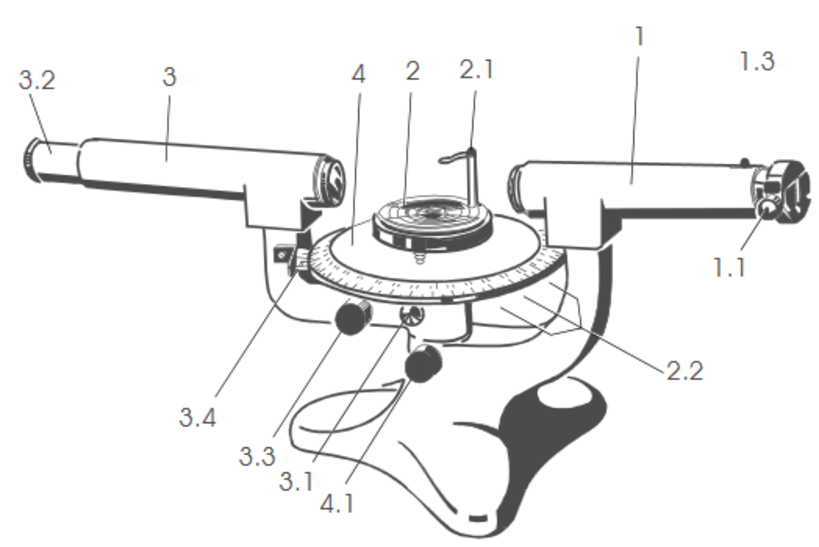
\includegraphics{ressources/Aufbau.pdf}
  \caption{Aufbau des Okularmikrometers \cite{skript}.}
  \label{fig:Aufbau}
\end{figure}

\subsection{Winkelbeziehungen am Reflexionsgitter}
\label{sec:winkelbeziehungen}
In Abbildung \ref{fig:winkel} sind alle relevanten Winkelbeziehungen eingezeichnet.
\begin{figure}
  \centering
  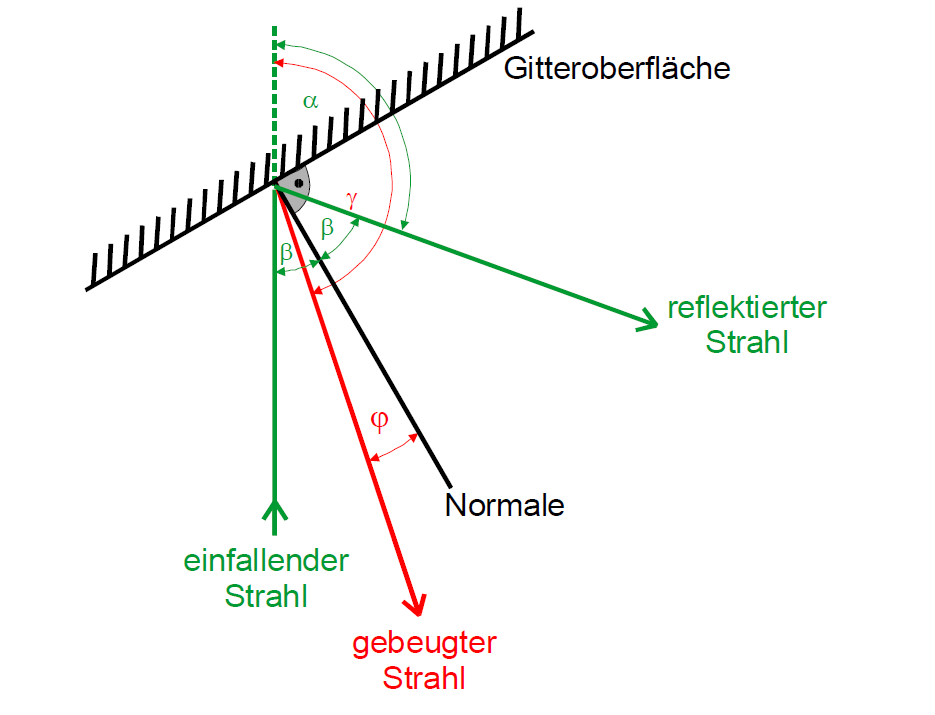
\includegraphics[width=0.6\textwidth]{ressources/Winkel.png}
  \caption{Winkelbeziehungen beim Reflexionsgitter \cite{skript}.}
  \label{fig:winkel}
\end{figure}
Es gilt für den Reflexionswinkel zum Lot
\begin{equation}
  \beta = 90\si{\degree} - \frac{400\si{\degree} - \delta}{2}
\end{equation}
und für den Beugungswinkel zum Lot
\begin{equation}
  \varphi = 400\si{\degree} - \delta' + \beta - 180 \si{\degree} \; .
\end{equation}
Hierin sind $\delta$ und $\delta'$ die an der Teilkreisscheibe abgelesenen Winkel. Für diese Zusammenhänge wird aus Gleichung \eqref{eq:sinphi} mit $k=1$ dann
\begin{equation}
  \sin{\varphi} = k\frac{\lambda}{g} - \sin{\beta}  \; .
\end{equation}
